\chapter{Implementation}

Ce chapitre reprend un ensemble de   technologies destinées  à la manipulation des données massives. Ce sont les technologies que nous avons utilisé pour analyser les traceroutes disponibles dans le dépôt de RIPE Atlas. Nous allons présenter l'objectif de chaque technologie, ses avantages, ses inconvénients et ses limitations dans le cas de la présente analyse.


\section{MongoDB}


\paragraph{Introduction à la base de données MongoDB} \label{subsubsection:mongodb}~

MongoDB\footnote{Source : \url{https://www.mongodb.com/}, consultée le $02/08/2018$.} est une base de données  NoSQL de type Document\footnote{Une base de données NoSQL de type document est décrite dans la section \ref{sec:nosql-database}.}.  MongoDB est classé parmi les  SGBD adoptant le couple CP (Consistency-Partition Tolerance) dans le théorème  CAP\footnote{Le théorème  CAP est décrit dans la section \ref{par:cap-theorem}}. Une base de données créées dans MongoDB est un ensemble de collections\footnote{Une collection dans MongoDB est équivalente à une table dans un SGBDR.}.

En $ 2016 $, MongoDB devient disponible en mode cloud sous le nom  MongoDB Atlas \footnote{Source : \url{https://www.mongodb.com/cloud/atlas}, consultée le $ 02/08/2018 $.}.  Il est distribué à travers les trois fournisseurs du cloud: Amazon Web Services (AWS), Google Cloud Platform et Microsoft Azure.  En terme de tarifs, plusieurs formules sont proposées \footnote{Source : \url{https://www.mongodb.com/cloud/atlas/pricing}, consultée le $ 02/08/2018 $.}, y inclut l'offre gratuite pour expérimenter MongoDB Atlas.  Les frais d'utilisation du service MongoDB Atlas dépend du stockage, de la  RAM allouées et des options choisies.

\paragraph{Application sur les  traceroutes }~

Les données relatives aux mesures traceroutes peuvent être récupérées de différentes manières. Par exemple,  les traceroutes à destination des instances du serveur DNS K-root. En ce qui concerne le travail de référence, les traceroutes sont récupérés à la fois par type d'adressage : IPv4 et IPv6 en se basant sur  l'identifiant  de la mesure : $ 5001 $, $ 6006 $, etc et par date.  Ainsi les traceroutes sont organisés, dans MongoDB, dans des collections.  Chaque collection stocke les traceroutes effectués lors de la journée $YYYY\_MM\_DD$ et en adressage $V$. $V$ est vide en cas d'adressage IPv4 et $V$ égal à $6$ s'il s'agit de l'adressage IPv6. La nomination structurée permet de ne récupérer que les traceroutes concernés. Chaque collection contient un ensemble de traceroutes formatés en format BSON. Ainsi, le nom d'une collection est structuré comme suit: 	$tracerouteV\_YYYY\_MM\_DD$.

\begin{tcolorbox}
BSON (ou Binary JSON) est un format utilisé pour stocker et transférer les données dans la base de données MongoDB. BSON facilite la représentation des structures de données simples et des tableaux associatifs\footnote{Source : \url{https://fr.wikipedia.org/wiki/BSON}, consultée le $ 02/08/2018 $.}.
\end{tcolorbox}
\paragraph{Les limitations du MongoDB}

L'implémentation proposée de l'outil de détection utilise la version locale de la base de données MongoDB pour le stockage des données.  La quantité de données dont MongoDB peut stocker dépend de l'espace mémoire de stockage disponible dans la machine dans laquelle MongoDB est installé. De plus, les performances d'une détection lancée concernant une période donnée dépendent de l'espace mémoire vive libre dans la machine en question. Pour conclure, l'utilisation la version locale du MongoDB pour analyser les traceroutes à travers l'outil de détection dépend typiquement de la machine locale.


\section{DynamoDB}

 \paragraph{Amazon DynamoDB :}\label{aws:dynmo}~

Amazon DynamoDB\footnote{Source : \url{https://aws.amazon.com/fr/dynamodb/}, consultée le $02/05/2018$.} est une base de données NoSQL de type clé-valeur distribuée, gérée par les services d'Amazon. Elle est capable de stocker un volume important de données limité par la capacité de l'infrastructure d'AWS. Amazon DynamoDB   est simple et facile à utiliser,  elle ne nécessite aucune configuration préalable. 

Amazon DynamoDB  est une base de données évolutive de façon abstraite pour l'utilisateur final. Elle offre des performances constantes à une échelle essentiellement infinie, limitée uniquement par la taille physique du cloud AWS. Elle est flexible. Aucun schéma n'est requis pour stocker les données. Les frais d'utilisation de ce service dépendent de trois éléments\footnote{Source : \url{https://aws.amazon.com/fr/dynamodb/pricing/}, consultée $02/05/2018$.}:
\begin{itemize}
	\item[--] la quantité de données stockées : DynamoDB est facturé par Go d'espace disque utilisé ($ 0,250 $ USD par Go par mois);
	\item[--] la capacité en lecture par seconde ($ 0,470 $ USD par unité de capacité d'écriture par mois);
	\item[--]  la capacité en écriture par seconde ($ 0,090 $ USD par unité de capacité de lecture par mois);
\end{itemize}


\paragraph{Application sur les traceroutes}~


L'évolutivité est une des caractéristiques attirantes d'Amazon DynamoDB. Nous n'avons pas à se soucier des limitations en terme d'espace disponible de stockage. Toutefois, le problème peut se poser au niveau de la récupération et de la manipulation de ces données. Prenant l'exemple de l'analyse des traceroutes, si on souhaite analyser tout les traceroutes effectués durant une heure du temps, il faut ajuster les ressources de la machine qui accueille ces données afin d'assurer le bon déroulement de détection. A titre indicatif, une heure de traceroutes fait en moyen $620$ MB en format compressé (environ $9$ GB).




\section{Amazon S3, Amazon Athena et Amazon Glue }

Il existe un ensemble de services web proposés par Amazon  adaptés à la manipulation des données massives. Le deuxième choix a été dirigé vers une combinaison de services d'Amazon, il s'agit d'Amazon S3, Amazon Glue et Amazon Athena.

\paragraph{Introduction aux services Amazon S3, Amazon Athena et Amazon Glue }

\subparagraph{Amazon S3}
\footnote{Source : \url{https://aws.amazon.com/fr/s3/}, consultée le $06/07/2018$.} est un service de stockage d'objets dans le cloud. Il est conçu pour stocker et  récupérer toute quantité de données. Il peut assurer $ 99,999999999 $ \% de durabilité. La sécurité  et l'accès aux données sont assurés. Il existe plusieurs classes de stockage qui répondent aux différents besoins. 


Les fichiers des données sont organisés dans ce qu'on appelle un compartiment, c'est une simulation de dossier dans un système d'exploitation. A l'intérieur d'un compartiment, il est possible de créer des compartiments imbriqués. C'est une simulation d'arborescence de dossiers car physiquement cet arborescence n'existe pas. En ce qui concerne les frais du service AWS S3, le tableau   	\ref{tab:pricing-s3-standard} illustre les tarifs de la formule standard.
\begin{table}[H]
	\centering
	\captionsetup{justification=centering}
	\begin{tabular}{l c }
		\textbf{Région} & UE (Irlande) \\ \hline
		\textbf{Première tranche de $ 50 $ To/mois} &	$ 0,023 $ USD par Go\\ \hline
		\textbf{$ 450 $ To suivants/mois} &	$ 0,022 $ USD par Go \\ \hline
		\textbf{Plus de $ 500 $ To/mois} &	$ 0,021 $ USD par Go\\ \hline
	\end{tabular}
	\caption{Les tarifs du AWS S3 (formule Stockage standard S3)}
	\label{tab:pricing-s3-standard}
	\source{\url{https://aws.amazon.com/fr/s3/pricing/}, consultée le $05/08/2018$.}
\end{table}

  
\subparagraph{Amazon  Glue} \label{aws:glue}
 \footnote{Source : \url{https://aws.amazon.com/fr/glue/}, consultée le $06/07/2018$.} est un service d'extraction, de transformation et de chargement. L'objectif de ce service est de découvrir les données, les transformer et les rendre accessibles à la recherche et à l'interrogation.  Amazon Glue  est utile pour la construction des entrepôts de données; il découvre les métadonnées relatives aux magasins de données et les rendre accessibles dans un catalogue central. En prenant en entrée les données  présentes dans un compartiment dans Amazon S3, Amazon Glue découvre le schéma de ces données. Il dispose de plusieurs classificateurs intégrés pour la découverte des données. Par exemple un classificateur pour trouver le schéma  des données en format JSON, XML, etc. Si les classificateurs intégrés ne répondent pas aux besoins particuliers, il est possible de créer des classificateurs personnalisables. 

Les frais de ce service dépendent du temps écoulé lors de l'analyse des données par les robots d'analyse durant la découverte du schéma. A ces frais, ils s'ajoutent les frais du catalogue de données qui va être peuplé par les résultats fournis par les robots d'analyse. Par exemple, on paye $ 0,44 $ USD par heure par DPU\footnote{DPU : unité de traitement des données.}, il est facturé à la seconde avec un minimum de $ 10 $ minutes par robot d'analyse exécuté. Plus de détails sont disponibles sur Amazon Glue\footnote{Source : \url{https://aws.amazon.com/fr/glue/pricing/}, consultée le $05/08/2018$.}.

\subparagraph{Amazon Athena}\label{aws:athena}\footnote{Source : \url{https://aws.amazon.com/fr/athena/}, consultée le $06/07/2018$.} est un service de requêtes  interactif. Il permet d'interroger les données présentes dans Amazon S3 avec des requêtes SQL plus avancées. Le service Amazon Athena est considéré comme \textit{serverless}. Amazon Athena utilise l'approche \textbf{\textit{schema-on-read}} (voir la section \ref{sec:schema-read-write}) afin de projeter le schéma donné en entrée sur les données au moment de l'exécution de la requête SQL demandée. Le schéma sur lequel les données peuvent être projetées peut être créé manuellement ou bien utiliser le catalogue créé dans Amazon Glue.
 Le service Amazon Athena est facturé suivant la quantité de données analysée. Précisément, $ 5 $ USD par To de données analysées.


\begin{tcolorbox}
	Une \textbf{\textit{requête est	interactive}} si on peut  obtenir immédiatement une réponse à la requête.  Dans le cas échéant, les résultats sont obtenus  dans le cadre d'un code source pour un des langages de programmation, souvent à travers une API.
\end{tcolorbox}

\begin{tcolorbox}
	\textbf{\textit{Serverless}} peut être décomposé en \textit{server} et \textit{less}. Un outil est \textit{serverless} quand l'utilisateur final de cet outil peut l'utiliser sans se soucier de toute configuration ou gestion des serveurs derrière ce service. C'est un mécanisme présent beaucoup sur le cloud.
\end{tcolorbox}

L'exécution des requêtes SQL est effectuée par le moteur de requêtes SQL Presto. pour les instruction DDL, elles sont effectuées par  \textit{Hive Data Definition Language} \footnote{Source : \url{https://cwiki.apache.org/confluence/display/Hive/LanguageManual+DDL}, consultée le $05/08/2018$.}. Les requêtes DDL incluent la création, la suppression et la mise à jour de la structure de la table dans le cas d'une base de données relationnelles, d'une collection, d'une vue, etc. 



\begin{tcolorbox}
	\textbf{\textit{Presto\footnote{Source : \url{http://prestodb.io/}, consultée le $01/08/2018$.} }} est un moteur de requêtes SQL open source destiné au Big Data. Il permet d'exécuter des requêtes analytiques interactives sur des données de taille importante; jusqu'à des Pétaoctets de données.
	
	Presto interroge les données où elles sont hébergées. Ce qui inclut les bases de données relationnelles, Amazon S3 et autres dépôts propriétaires. De plus, une même requête SQL peut combiner plusieurs sources de données. C'est intéressant pour les organisations ayant plusieurs sources de données. Il fournit les résultats en quelques secondes, voire quelques minutes.  Il supporte les types de données complexes comme les objets JSON, un tableau d'éléments, etc. Il supporte aussi  des opérations complexes sur les données.
\end{tcolorbox} 


\begin{tcolorbox}
	\textbf{Hive Data definition language} (DLL) est un sous-ensemble de déclarations qui décrivent la structure de données dans Apache Hive.  Principalement, ce sont les instruction de création, suppression et de mise à jour de la structure des objets comme les bases de données, les tables, les vues et autres.
\end{tcolorbox}

\paragraph{Application sur les traceroutes}~

Afin d'utiliser Amazon Athena, nous avons besoin du schéma des données. Il s'agit d'une table comme les tables dans un SGBDR. Pour ce faire, 
nous avons lancé, avec Amazon Glue,  la détection du schéma d'un ensemble de  traceroutes enregistrés dans un fichier faisant $500$ MB. Toutefois, la détection a échoué. Autrement dit, Amazon Glue n'a pas pu inférer le schéma d'une seule table capable de lire tout traceroute dans ce fichier.  L'échec de l'inférence est du au fait que le fichier contient des traceroutes différents en terme de structure. L'origine de cette différence  est le fait que ces traceroutes ont été effectués par des sondes ayant un firmware différent. Car le contenu des résultats d'une requête traceroute  et son organisation dans un objet JSON dépend partiellement du firmware de la sonde. C'est pourquoi nous avons créé le schéma des traceroutes manuellement (voir la section \ref{creer-table-traceroute} dans l'annexe \ref{athena-appendix}). La table a été créée en utilisant le partitionnement des données dans un compartiment S3. Plus de détails sur le partitionnement sont données dans la section \ref{subsubsection:partitionnement} dans l'annexe \ref{athena-appendix}.


Une fois les fichiers de données sont synchronisés vers le compartiment AWS S3 et le schéma  de données est créé, on passe à l'interrogation de données en utilisant les requêtes SQL basées sur Presto.  On distingue deux possibilités. La première possibilité n'utilise Athena que pour récupérer, dans la machine locale,  les traceroutes vérifiés en terme de validité (étape $1$ et $2$ dans \ref{steps-rtt-analysis} ).  Les traitements qui suivent (étapes  à partir de $3$) sont effectués dans la machine locale. Dans ce cas, l'utilisation des technologies du Big Data est limité qu'au niveau stockage de données massives. En ce qui concerne la deuxième possibilité, l'idée est de maximiser les traitements au niveau d'Athena, de ce fait, la machine locale n'a qu'à recevoir les derniers résultats.




En partant de la deuxième possibilité, les données doivent être interrogées de sorte à maximiser,  	au niveau d'Amazon Athena,  les traitements relatives aux étapes décrites dans la section \ref{steps-rtt-analysis}. Ainsi le défi est de trouver la requête ou bien l'ensemble de requêtes SQL à exécuter sur Athena en vue d'avoir l'évolution du RTT différentiel d'un lien donné.

Supposons qu'il existe une requête SQL capable de trouver les liens possibles avec leur RTT différentiel. A l'étape 4 dans \ref{steps-rtt-analysis}, on construit la distribution des RTTs différentiels pour tout lien $l$ identifié dans les traceroutes de la période $d_i$. Cette distribution est mise à jour à chaque $l$  identifié dans un des traceroutes  de la période $d_i$. Soient  $T_i$ = \{$t_{i, j}$\}  l'ensemble de traceroutes effectués durant $d_i$,  $j \in [1, R]$ et R est le nombre de traceroutes durant $d_i$. On peut décrire le parcours des traceroutes brièvement dans le pseudo-code suivant, sachant que les détails ne sont données, l'objectif est illustré la convenance d'Athena au traitement souhaité :
\begin{algorithm}[H]
\begin{algorithmic}[1]
	 \ForAll{ $t_{i, j}$ $\in$ $T_i$} \
	  \State $links$ $\leftarrow$ getLinksFromTraceroute($t_j$)
	  	 \ForAll{$l$ $\in$ $links$}
	  	 		\State updateLinkRttDistribution($l$) \label{update-link}
	  	 \EndFor
	 \EndFor
\end{algorithmic}
\caption{Une partie l'étape 4 du processus de la détection des anomalies des délais }
\label{alo-inference-link}
\end{algorithm}

\textit{getLinksFromTraceroute($t_j$)} énumère tous les liens possibles dans le traceroute $t_j$.
\textit{updateLinkRttDistribution($l$)} ajoute le RTT différentiel du lien $l$, précédemment calculé, à la distribution des RTTs différentiels courante.

Le service Athena est conçu pour la lecture de données, toute mise à jour de données n'est pas possible avec ce service. C'est pourquoi la distribution des RTTs différentiels de chaque  lien identifié doit être sauvegardée dans un endroit accessible en lecture et en écriture, par exemple dans un compartiment AWS S3. Que ce soit un fichier reprenant la distribution des RTTs différentiel  par un seul lien ou bien un fichier pour tous les liens,   à la ligne  \ref{update-link} du pseudo-code \ref{alo-inference-link}, un fichier doit être lu et mise à jour avec de nouvelle valeur.

Pour une $d_i$ d'une heure, le nombre de traceroutes est de l'ordre des milliers. Chaque traceroute peut inclure $L$ liens. Dans ce cas, le nombre de mise à jour de la distribution des RTTs différentiels est $R$\texttimes$L$. Avec une autre technologie qui travaille en mémoire, les résultats sont données plus rapidement. 







\section{Spark Apache avec Scala}

\subsection{Introduction à Apache Sprk}

Apache Spark est un moteur de traitement distribué des données. Spark est conçu pour assurer la rapidité, la facilité d'utilisation ainsi que la flexibilité.

\paragraph{Spark Core Concepts et architecture}

\subparagraph{Spark Clusters et Resource Management System}

Spark est un système distribué conçu pour traiter les données massives rapidement et avec efficacité. Ce système est déployé sur un ensemble de machines, qu'onappelle Spark \textit{cluster}. La taille du cluster en nombre de machines est variable, il existe un cluster avec peu de machines mais aussi un cluster avec des milliers de machines. En vue de gérer efficacement les machines d'un cluster, les entreprises recourent à un système de gestion de ressources tel que Apache YARN\footnote{Description dans \url{https://hadoop.apache.org/docs/current/hadoop-yarn/hadoop-yarn-site/YARN.html}, consulté le $09/12/2018$.} ou Apache Mesos\footnote{Site officiel \url{https://mesos.apache.org/}, consulté le $09/12/2018$.}. Les deux composantes les plus importantes dans un système de gestion de ressources sont : le \textit{cluster manager} et le \textit{worker}.

Le \textit{cluster manager} a une vue globale de l'emplacement des workers, la mémoire qu'ils ont et le nombre de c\oe{}urs CPU dont chaque worker dispose. Le rôle du \textit{cluster manager} est d'orchestrer le travail en le désignant à chaque worker. La Figure \ref{fig:cluster-overview} montre l'interaction entre le cluster manager et les workers.


\begin{figure}[H]
	\centering
	\captionsetup{justification= centering}
	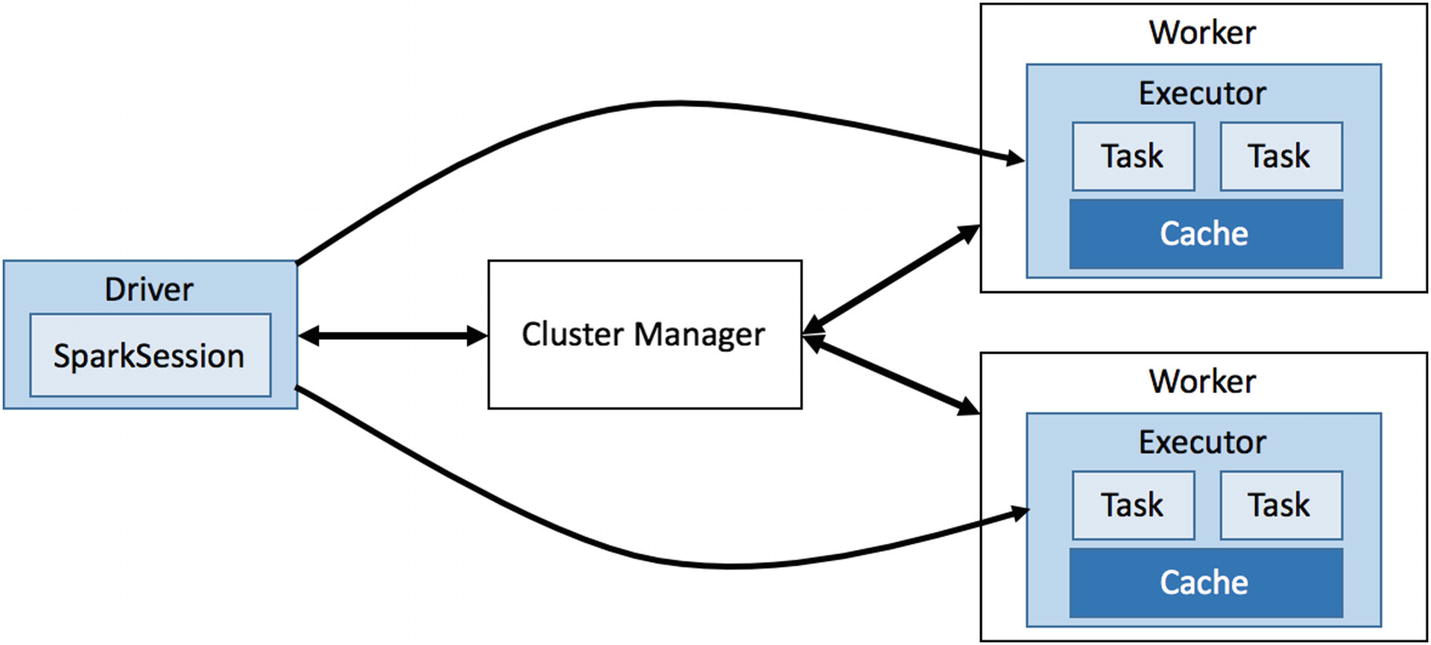
\includegraphics[width=0.7\linewidth]{illustrations/cluster-overview.jpg}
	\caption{ Interaction entre une application Spark et le cluster manager. Source : \cite{eginning-Apache-Spark-2-cluster-overwiew}}
	\label{fig:cluster-overview}
\end{figure}




\subparagraph{Spark Application}
Une application Spark consiste en deux parties. La première partie concerne la logique décrivant les traitements à appliquer sur les données.  Cette logique est décrite à travers les APIs\footnote{API en Java, Scala, Python ou R.} disponibles. La deuxième partie est appelée le \textit{driver}, c'est le coordinateur principal d'une application Spark. Le driver interagit avec le cluster manager afin de trouver les machines sur lesquelles le traitement de données doit être réalisé. Ainsi, pour chacune de ces machines, le driver Spark lance le processus \textit{executor} en passant par le cluster manager. Un autre rôle du le driver Spark est de gérer et de distribuer les tâches Spark en provenance de l'application Spark sur chaque executor. Pour précision, le point d'entrée vers une application Spark est la class \textit{SparkSession}.

\subparagraph{Spark driver et executor}

Chaque Spark executor est alloué exclusivement à une application Spark spécifique et la durée de vie d'un executor est celle de l'application Spark. 

Spark utilise l'architecture master-slave. Spark driver est le master et Spark executor est le slave. De ce fait, une application Spark n'a qu'un seul Spark driver et plusieurs Spark executors. Chaque Spark executor s'occupe d'un traitement  sur une partie de données. Ainsi Spark permet de traiter  les données de manière parallèle. La Figure \ref{fig:small-cluster-3} illustre un exemple d'un cluster. Ce dernier est composé de trois executors.
\begin{figure}[H]
	\centering
	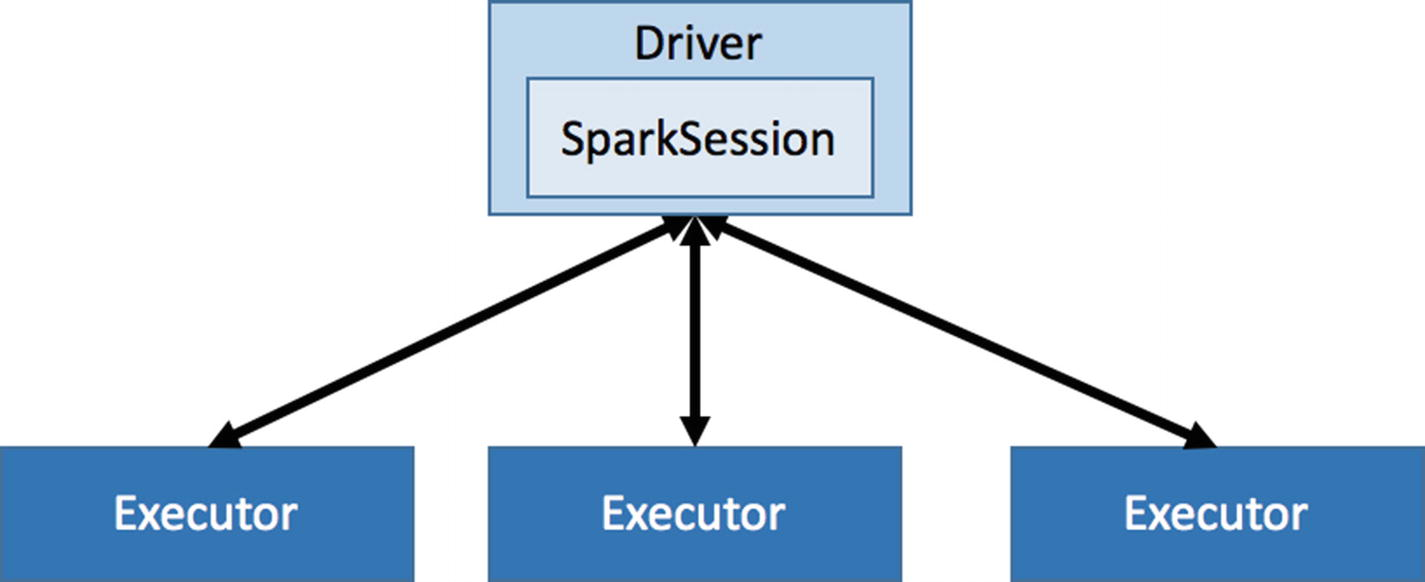
\includegraphics[width=0.7\linewidth]{illustrations/small-cluster-3}
	\caption{Un exemple d'un cluster formé de trois executors. Source : \cite{eginning-Apache-Spark-2-cluster-example}}
	\label{fig:small-cluster-3}
\end{figure}


\subparagraph{Spark Uniffied Stack} Spark offre ce qu'on appelle Spark Stack. C'est un ensemble de composantes construites dessus la composante Spark Core.  Ces composantes sont conçues pour répondre à des besoins spécifiques :
\begin{itemize}
	\item Spark SQL  est conçu pour le traitement interactive;
	\item Spark Streaming est utilisé pour les traitements en temps réel;
	\item  GraphX est destiné au traitement de graphe;
	\item MLib est conçu pour le machine learning;
	\item SparkR est consacré au traitement lié au machine learning en utilisant l shell R.
	
\end{itemize}

\subparagraph{Spark Core} est la base du moteur Spark pour e traitement distribué de données.  On distingue deux parties formant Spark Core. Premièrement, la partie concernant l'infrastructure distribué du calcul. Cette dernière est responsable de la distribution, la coordination et la planification des tâches  sur les différentes machines formant le cluster. De plus, cette partie gère l'échec d'un traitement donnée et le transfert de donnés entre les machines. Le deuxième élément formant Spark Core est appelé RDD (Resilient Distributed Dataset). Un RDD est une collection partitionnée d'objets, tolérant au pannes et en lecture seule. 
La Figure \ref{fig:unified-stack} 

\begin{figure}[H]
	\centering
	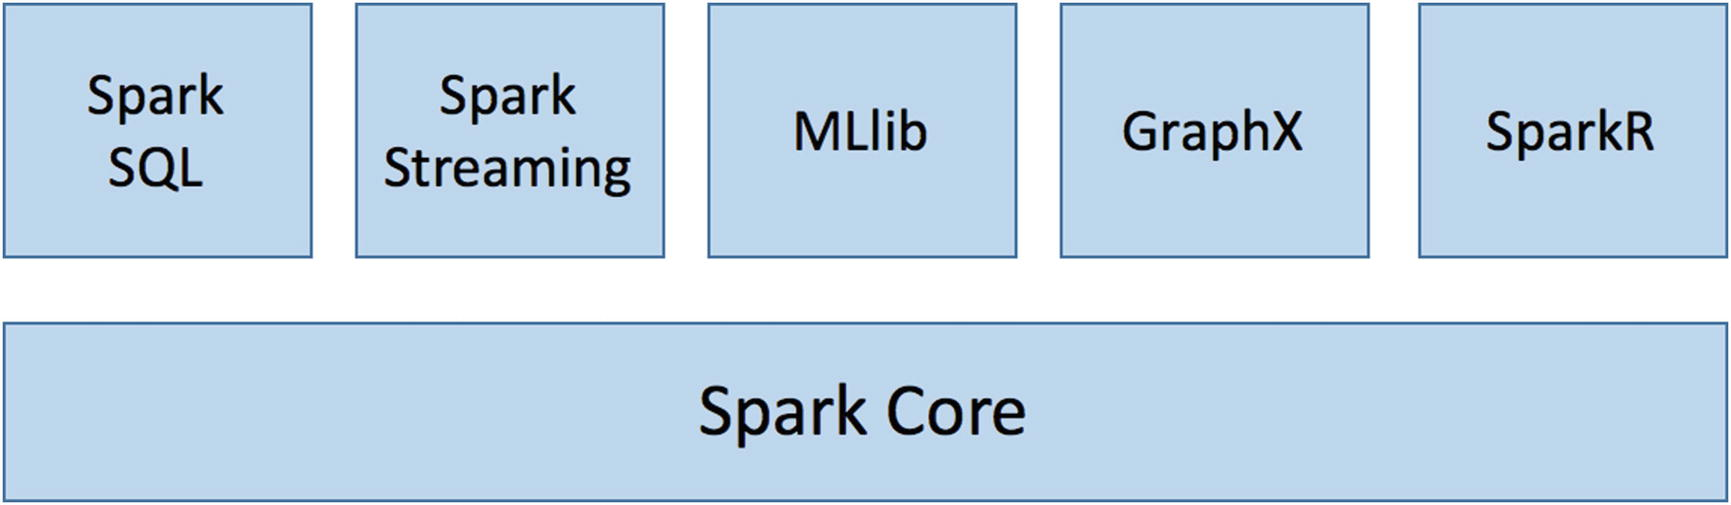
\includegraphics[width=0.7\linewidth]{illustrations/unified-stack}
	\caption{ Spark Unified Stack. Source : \cite{eginning-Apache-Spark-2-unified-stack}}
	\label{fig:unified-stack}
\end{figure}





\subsection{Application sur traceroutes}
%\subsection{Complément d'information du processus de la détection avec le langage Scala}
Comme complément aux étapes décrites dans \ref{steps-rtt-analysis}, on présente les différentes classes permettant de modéliser les données tout au long du processus de l'analyse. La définition de ces classes est liée au langage \textit{Scala}. 

Soient les classes suivantes utilisées : 

\paragraph{La classe Signal} modélise un signal \footnote{Un signal dans le contexte d'un traceroute.}. Ainsi, \textit{from} est l'adresse IP du routeur émettant ce signal, \textit{rtt} est le Round Trip Time entre la sonde Atlas et ce routeur et enfin \textit{x} est un indicateur de l'échec du signal.
\begin{lstlisting}[language=scala]
case class Signal(
rtt:  Option[Double],
x:    Option[String],
from: Option[String])
\end{lstlisting}

\paragraph{La classe Hop} modélise un saut dans un traceroute. On caractérise un saut par son identifiant noté \textit{hop}. Celui-ci   prend comme valeur un entier commençant à $1$ et la liste des signaux relatifs à ce saut notée par \textit{result}. Généralement un saut est représenté par $3$ signaux.
\begin{lstlisting}[language=scala]
case class Hop(
var result: Seq[Signal],
hop:        Int)
\end{lstlisting}
\paragraph{La classe Traceroutes} modélise le résultat d'une requête traceroute effectuée par une sonde Atlas. Cette modélisation se limite aux données qui nous intéressent dans la présente analyse. 

\textit{dst\_name} représente l'adresse IP de la destination de la requête traceroute, \textit{from} est l'adresse IP de la sonde, \textit{prb\_id} est l'identifiant de la sonde, \textit{msm\_id} est l'identifiant de mesure, \textit{timestamp} est le temps auquel la requête traceroute a été effectuée et enfin on trouve la liste des sauts qui représentent les routeurs traversés par le trafic entre la source et la destination. 

\begin{lstlisting}[language=scala]
case class Traceroute(
dst_name:  String,
from:      String,
prb_id:    BigInt,
msm_id:    BigInt,
timestamp: BigInt,
result:    Seq[Hop])
\end{lstlisting}
\paragraph{La classe TraceroutesPerPeriod} permet de présenter les traceroutes après les avoir trié   suivant la période pendant laquelle ils ont été effectués.   \textit{timeWindow} est le temps unix marquant le début de la période \footnote{Pour précision, la fin de la période peut être inférée en prenant deux débuts de deux périodes car la durée d'une période est fixe tout au long de l'analyse.} et  \textit{traceroutes} est la liste des traceroutes effectués pendant cette période. 


A l'étape 2, l'objectif était d'agréger  les signaux par routeur source et ensuite calculer la médiane des RTTs par ce routeur. Par conséquent, un traceroute est présenté différemment, ce qui est  illustré par la classe \textit{MedianByHopTraceroute}.

\paragraph{La classe PreparedSignal }  est une agrégation de tous les signaux, d'un saut donné, par le routeur \textit{from},  la médiane des RTTs calculée est présentée par \textit{medianRtt}.
\begin{lstlisting}[language=scala]
case class PreparedSignal(
medianRtt: Double,
from:      String)
\end{lstlisting}
\paragraph{La classe PreparedHop } modélise un saut après avoir agrégé ses signaux. 
\begin{lstlisting}[language=scala]
case class PreparedHop(
var result: Seq[PreparedSignal],
hop:        Int)
\end{lstlisting}


\paragraph{La classe MedianByHopTraceroute } modélise un traceroute après avoir agrégé ses sauts. Par rapport au traceroute d'avant l'agrégation, seule la liste des sauts  a subi un changement. 
\begin{lstlisting}[language=scala]
case class MedianByHopTraceroute(
dst_name:  String,
from:      String,
prb_id:    BigInt,
msm_id:    BigInt,
timestamp: BigInt,
result:    Seq[PreparedHop])
\end{lstlisting}


\paragraph{La classe Link} modélise un lien topologique. Ce dernier est défini par deux adresses IP  \textit{ip1} et \textit{ip2} et par son RTT différentiel calculé \textit{rttDiff}.
\begin{lstlisting}[language=scala]
case class Link(
ip1:     String,
ip2:     String,
rttDiff: Double)
\end{lstlisting}

\paragraph{La classe LinksTraceroute} permet de modéliser un traceroute après avoir inféré tous les liens de ce dernier. Ainsi, la liste des sauts est remplacée par la liste des liens (\textit{links}). 

\begin{lstlisting}[language=scala]
case class LinksTraceroute(
dst_name:  String,
from:      String,
prb_id:    BigInt,
msm_id:    BigInt,
timestamp: BigInt,
links:     Seq[Link])
\end{lstlisting}


A l'étape 5, l'objectif était de passer d'un traceroute à une liste de liens caractérisés par les informations générales sur la sonde Atlas, la mesure Atlas, etc. Chaque élément de cette liste est représenté par la classe \textit{DiffRtt}, où \textit{LinkIPs} représente les deux adresses IP d'un lien donné.
\paragraph{La classe LinkIPs} permet représenter un lien par seulement ses deux adresses IP \textit{ip1} et \textit{ip2}.
\begin{lstlisting}[language=scala]
case class LinkIPs(
ip1: String,
ip2: String)
\end{lstlisting}

\paragraph{La classe DiffRtt} est une représentation plus détaillée d'un lien, en plus de son RTT différentiel, on ajoute d'autres informations.  Les adresses IP d'un lien sont modélisées par la classe \textit{LinkIPs}.

\begin{lstlisting}[language=scala]
case class DiffRtt(
rtt:      Double,
var link: LinkIPs,
probe:    BigInt)
\end{lstlisting}

A l'étape 6.3, on souhaite normaliser les dates de chaque lien; peu importe le moment pendant lequel le traceroute a été effectué durant une période $d_i$, on note seulement le début de cette période. Ainsi,  la classe  \textit{DiffRTTPeriod}  reprend un \textit{lien} donné, les différentes sondes Atlas ayant identifié ce lien (\textit{probes}), les RTTs différentiels de ce lien tout au long de la période et enfin les dates associées à chaque RTT différentiel.
\paragraph{La classe DiffRTTPeriod } ~
\begin{lstlisting}[language=scala]
case class DiffRTTPeriod(
link:      LinkIPs,
probes:    Seq[BigInt],
rtts:      Seq[Double],
var dates: Seq[Int])
\end{lstlisting}

A la fin des opérations de l'étape 6, on reprend pour chaque période, pour un lien donné, les RTTs différentiels ainsi que leurs dates. Ensuite, on construit les bornes de l'intervalle de confiance courants pour ce lien et les bornes de l'intervalle de confiance de référence, et ce afin de comparer ces deux intervalles en vue d'inférer les anomalies possibles du délais de ce lien.


\paragraph{La classe LinkState } permet de modéliser les intervalles de confiance d'un lien pendant une période $d_i$ donnée. \textit{valueLow} est la borne inférieur de l'intervalle de confiance, \textit{valueHi} est la borne supérieure de l'intervalle de confiance, \textit{valueMedian} est la médiane des RTTs différentiels et enfin \textit{valueMean} est la moyenne des RTTs différentiels. Pour précision, les données concernant l'état d'un lien sont sous forme d'une liste. L'idée est de garder l'historique de ces valeurs durant toute la période de l'analyse. Cette historique est exploitée pour tracer l'évolution du RTT différentiel du lien. Cependant, la comparaison utilise les valeurs du dernier état du lien.

  

%Pour toute période, on a une instance de \textit{LinkState} pour 
\begin{lstlisting}[language=scala]
case class LinkState(
var valueMedian: Seq[Double],
var valueHi:     Seq[Double],
var valueLow:    Seq[Double],
var valueMean:   Seq[Double])
\end{lstlisting}
\paragraph{La comparaison des intervalles de confiance} 

La comparaison de l'état courant du lien avec celui de référence est effectuée en analysant le chevauchement d'intervalles de confiance  courant et de référence. Le délai d'un lien est jugé anormal si son intervalle de confiance courant est inclus dans l'intervalle de confiance de référence. C'est le cas 1 dans la Figure 	\ref{fig:intervals-comparaison},  \textit{referenceLow} et \textit{referenceHight} sont les bornes de l'intervalle de confiance de référence.  \textit{currentLow} et \textit{currentHight} sont les bornes de l'intervalle de confiance courant.

D'après le travail de référence, on distingue quatre cas possibles  illustrés dans la Figure 	\ref{fig:intervals-comparaison}:

\subparagraph{Cas 1 :} le délai du lien est normal.
\subparagraph{Cas 2 :} le délai du lien est anormal.
\subparagraph{Cas 3 :} le délai du lien est anormal.
\subparagraph{Cas 4 :} le délai du lien est anormal.

Dans le cas où le délai est jugé anormal, on introduit ce qu'on appelle la \textit{déviation}. Cette métrique caractérise l'anomalie détectée. Elle est calculée différemment dans le cas où le délai est anormal.

\begin{figure}[h]
	\centering
	\captionsetup{justification=centering}
	\resizebox{\textwidth}{!}{
	% Graphic for TeX using PGF
% Title: /home/hayat/RipeAtlasTraceroutesAnalysis/report/illustrations/intervals-comparaison.dia
% Creator: Dia v0.97+git
% CreationDate: Tue Dec  4 13:30:20 2018
% For: hayat
% \usepackage{tikz}
% The following commands are not supported in PSTricks at present
% We define them conditionally, so when they are implemented,
% this pgf file will use them.
\ifx\du\undefined
  \newlength{\du}
\fi
\setlength{\du}{15\unitlength}
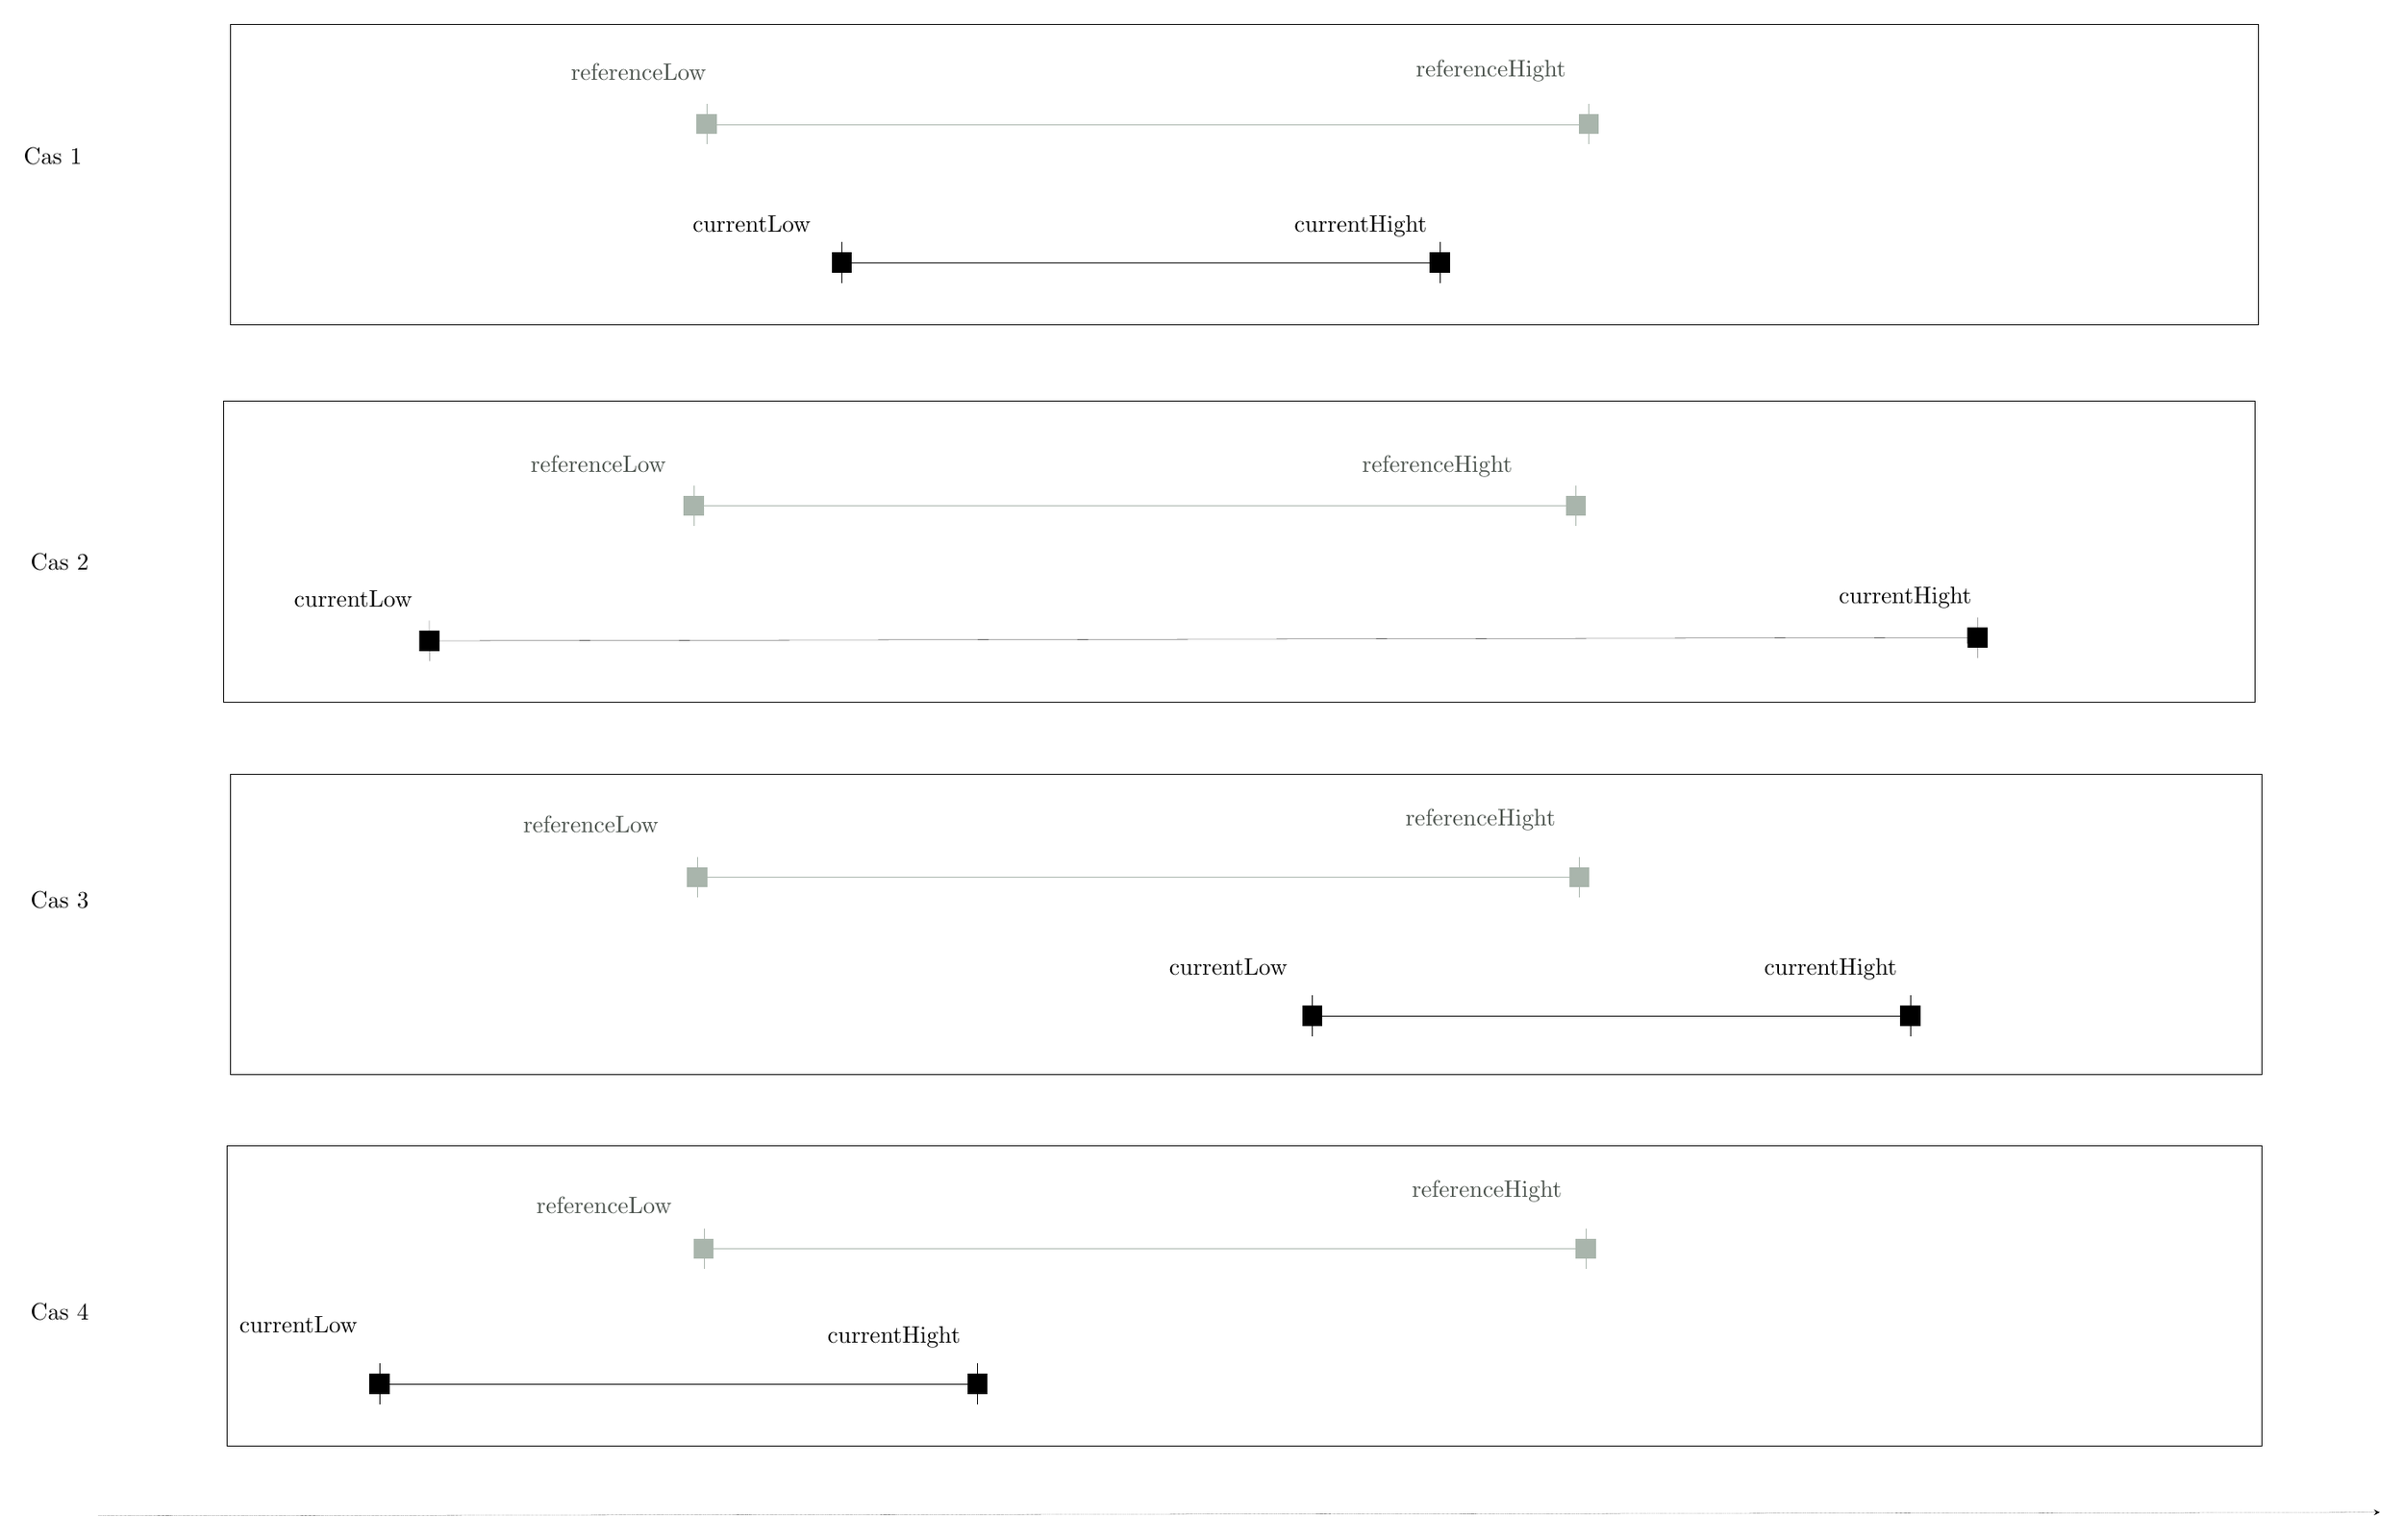
\begin{tikzpicture}[even odd rule]
\pgftransformxscale{1.000000}
\pgftransformyscale{-1.000000}
\definecolor{dialinecolor}{rgb}{0.000000, 0.000000, 0.000000}
\pgfsetstrokecolor{dialinecolor}
\pgfsetstrokeopacity{1.000000}
\definecolor{diafillcolor}{rgb}{1.000000, 1.000000, 1.000000}
\pgfsetfillcolor{diafillcolor}
\pgfsetfillopacity{1.000000}
\pgfsetlinewidth{0.100000\du}
\pgfsetdash{}{0pt}
\pgfsetbuttcap
{
\definecolor{diafillcolor}{rgb}{0.662745, 0.709804, 0.674510}
\pgfsetfillcolor{diafillcolor}
\pgfsetfillopacity{1.000000}
% was here!!!
}
\definecolor{dialinecolor}{rgb}{0.662745, 0.709804, 0.674510}
\pgfsetstrokecolor{dialinecolor}
\pgfsetstrokeopacity{1.000000}
\draw (14.150000\du,0.400000\du)--(27.000000\du,0.400000\du);
\pgfsetlinewidth{0.100000\du}
\pgfsetdash{}{0pt}
\pgfsetmiterjoin
\pgfsetbuttcap
\definecolor{diafillcolor}{rgb}{0.662745, 0.709804, 0.674510}
\pgfsetfillcolor{diafillcolor}
\pgfsetfillopacity{1.000000}
\fill (13.900000\du,0.550000\du)--(13.900000\du,0.250000\du)--(14.200000\du,0.250000\du)--(14.200000\du,0.550000\du)--cycle;
\definecolor{dialinecolor}{rgb}{0.662745, 0.709804, 0.674510}
\pgfsetstrokecolor{dialinecolor}
\pgfsetstrokeopacity{1.000000}
\draw (14.050000\du,0.700000\du)--(14.050000\du,0.100000\du);
\pgfsetlinewidth{0.100000\du}
\pgfsetdash{}{0pt}
\pgfsetmiterjoin
\pgfsetbuttcap
\definecolor{diafillcolor}{rgb}{0.662745, 0.709804, 0.674510}
\pgfsetfillcolor{diafillcolor}
\pgfsetfillopacity{1.000000}
\fill (27.250000\du,0.250000\du)--(27.250000\du,0.550000\du)--(26.950000\du,0.550000\du)--(26.950000\du,0.250000\du)--cycle;
\definecolor{dialinecolor}{rgb}{0.662745, 0.709804, 0.674510}
\pgfsetstrokecolor{dialinecolor}
\pgfsetstrokeopacity{1.000000}
\draw (27.100000\du,0.100000\du)--(27.100000\du,0.700000\du);
\pgfsetlinewidth{0.100000\du}
\pgfsetdash{}{0pt}
\pgfsetbuttcap
{
\definecolor{diafillcolor}{rgb}{0.000000, 0.000000, 0.000000}
\pgfsetfillcolor{diafillcolor}
\pgfsetfillopacity{1.000000}
% was here!!!
}
\definecolor{dialinecolor}{rgb}{0.000000, 0.000000, 0.000000}
\pgfsetstrokecolor{dialinecolor}
\pgfsetstrokeopacity{1.000000}
\draw (16.150000\du,2.450000\du)--(24.800000\du,2.450000\du);
\pgfsetlinewidth{0.100000\du}
\pgfsetdash{}{0pt}
\pgfsetmiterjoin
\pgfsetbuttcap
\definecolor{diafillcolor}{rgb}{0.000000, 0.000000, 0.000000}
\pgfsetfillcolor{diafillcolor}
\pgfsetfillopacity{1.000000}
\fill (15.900000\du,2.600000\du)--(15.900000\du,2.300000\du)--(16.200000\du,2.300000\du)--(16.200000\du,2.600000\du)--cycle;
\definecolor{dialinecolor}{rgb}{0.000000, 0.000000, 0.000000}
\pgfsetstrokecolor{dialinecolor}
\pgfsetstrokeopacity{1.000000}
\draw (16.050000\du,2.750000\du)--(16.050000\du,2.150000\du);
\pgfsetlinewidth{0.100000\du}
\pgfsetdash{}{0pt}
\pgfsetmiterjoin
\pgfsetbuttcap
\definecolor{diafillcolor}{rgb}{0.000000, 0.000000, 0.000000}
\pgfsetfillcolor{diafillcolor}
\pgfsetfillopacity{1.000000}
\fill (25.050000\du,2.300000\du)--(25.050000\du,2.600000\du)--(24.750000\du,2.600000\du)--(24.750000\du,2.300000\du)--cycle;
\definecolor{dialinecolor}{rgb}{0.000000, 0.000000, 0.000000}
\pgfsetstrokecolor{dialinecolor}
\pgfsetstrokeopacity{1.000000}
\draw (24.900000\du,2.150000\du)--(24.900000\du,2.750000\du);
\pgfsetlinewidth{0.100000\du}
\pgfsetdash{}{0pt}
\pgfsetbuttcap
{
\definecolor{diafillcolor}{rgb}{0.662745, 0.709804, 0.674510}
\pgfsetfillcolor{diafillcolor}
\pgfsetfillopacity{1.000000}
% was here!!!
}
\definecolor{dialinecolor}{rgb}{0.662745, 0.709804, 0.674510}
\pgfsetstrokecolor{dialinecolor}
\pgfsetstrokeopacity{1.000000}
\draw (14.008246\du,11.548114\du)--(26.858246\du,11.548114\du);
\pgfsetlinewidth{0.100000\du}
\pgfsetdash{}{0pt}
\pgfsetmiterjoin
\pgfsetbuttcap
\definecolor{diafillcolor}{rgb}{0.662745, 0.709804, 0.674510}
\pgfsetfillcolor{diafillcolor}
\pgfsetfillopacity{1.000000}
\fill (13.758246\du,11.698114\du)--(13.758246\du,11.398114\du)--(14.058246\du,11.398114\du)--(14.058246\du,11.698114\du)--cycle;
\definecolor{dialinecolor}{rgb}{0.662745, 0.709804, 0.674510}
\pgfsetstrokecolor{dialinecolor}
\pgfsetstrokeopacity{1.000000}
\draw (13.908246\du,11.848114\du)--(13.908246\du,11.248114\du);
\pgfsetlinewidth{0.100000\du}
\pgfsetdash{}{0pt}
\pgfsetmiterjoin
\pgfsetbuttcap
\definecolor{diafillcolor}{rgb}{0.662745, 0.709804, 0.674510}
\pgfsetfillcolor{diafillcolor}
\pgfsetfillopacity{1.000000}
\fill (27.108246\du,11.398114\du)--(27.108246\du,11.698114\du)--(26.808246\du,11.698114\du)--(26.808246\du,11.398114\du)--cycle;
\definecolor{dialinecolor}{rgb}{0.662745, 0.709804, 0.674510}
\pgfsetstrokecolor{dialinecolor}
\pgfsetstrokeopacity{1.000000}
\draw (26.958246\du,11.248114\du)--(26.958246\du,11.848114\du);
\pgfsetlinewidth{0.100000\du}
\pgfsetdash{}{0pt}
\pgfsetbuttcap
{
\definecolor{diafillcolor}{rgb}{0.000000, 0.000000, 0.000000}
\pgfsetfillcolor{diafillcolor}
\pgfsetfillopacity{1.000000}
% was here!!!
}
\definecolor{dialinecolor}{rgb}{0.000000, 0.000000, 0.000000}
\pgfsetstrokecolor{dialinecolor}
\pgfsetstrokeopacity{1.000000}
\draw (23.108246\du,13.598114\du)--(31.758246\du,13.598114\du);
\pgfsetlinewidth{0.100000\du}
\pgfsetdash{}{0pt}
\pgfsetmiterjoin
\pgfsetbuttcap
\definecolor{diafillcolor}{rgb}{0.000000, 0.000000, 0.000000}
\pgfsetfillcolor{diafillcolor}
\pgfsetfillopacity{1.000000}
\fill (22.858246\du,13.748114\du)--(22.858246\du,13.448114\du)--(23.158246\du,13.448114\du)--(23.158246\du,13.748114\du)--cycle;
\definecolor{dialinecolor}{rgb}{0.000000, 0.000000, 0.000000}
\pgfsetstrokecolor{dialinecolor}
\pgfsetstrokeopacity{1.000000}
\draw (23.008246\du,13.898114\du)--(23.008246\du,13.298114\du);
\pgfsetlinewidth{0.100000\du}
\pgfsetdash{}{0pt}
\pgfsetmiterjoin
\pgfsetbuttcap
\definecolor{diafillcolor}{rgb}{0.000000, 0.000000, 0.000000}
\pgfsetfillcolor{diafillcolor}
\pgfsetfillopacity{1.000000}
\fill (32.008246\du,13.448114\du)--(32.008246\du,13.748114\du)--(31.708246\du,13.748114\du)--(31.708246\du,13.448114\du)--cycle;
\definecolor{dialinecolor}{rgb}{0.000000, 0.000000, 0.000000}
\pgfsetstrokecolor{dialinecolor}
\pgfsetstrokeopacity{1.000000}
\draw (31.858246\du,13.298114\du)--(31.858246\du,13.898114\du);
\pgfsetlinewidth{0.100000\du}
\pgfsetdash{}{0pt}
\pgfsetbuttcap
{
\definecolor{diafillcolor}{rgb}{0.662745, 0.709804, 0.674510}
\pgfsetfillcolor{diafillcolor}
\pgfsetfillopacity{1.000000}
% was here!!!
}
\definecolor{dialinecolor}{rgb}{0.662745, 0.709804, 0.674510}
\pgfsetstrokecolor{dialinecolor}
\pgfsetstrokeopacity{1.000000}
\draw (14.108246\du,17.048114\du)--(26.958246\du,17.048114\du);
\pgfsetlinewidth{0.100000\du}
\pgfsetdash{}{0pt}
\pgfsetmiterjoin
\pgfsetbuttcap
\definecolor{diafillcolor}{rgb}{0.662745, 0.709804, 0.674510}
\pgfsetfillcolor{diafillcolor}
\pgfsetfillopacity{1.000000}
\fill (13.858246\du,17.198114\du)--(13.858246\du,16.898114\du)--(14.158246\du,16.898114\du)--(14.158246\du,17.198114\du)--cycle;
\definecolor{dialinecolor}{rgb}{0.662745, 0.709804, 0.674510}
\pgfsetstrokecolor{dialinecolor}
\pgfsetstrokeopacity{1.000000}
\draw (14.008246\du,17.348114\du)--(14.008246\du,16.748114\du);
\pgfsetlinewidth{0.100000\du}
\pgfsetdash{}{0pt}
\pgfsetmiterjoin
\pgfsetbuttcap
\definecolor{diafillcolor}{rgb}{0.662745, 0.709804, 0.674510}
\pgfsetfillcolor{diafillcolor}
\pgfsetfillopacity{1.000000}
\fill (27.208246\du,16.898114\du)--(27.208246\du,17.198114\du)--(26.908246\du,17.198114\du)--(26.908246\du,16.898114\du)--cycle;
\definecolor{dialinecolor}{rgb}{0.662745, 0.709804, 0.674510}
\pgfsetstrokecolor{dialinecolor}
\pgfsetstrokeopacity{1.000000}
\draw (27.058246\du,16.748114\du)--(27.058246\du,17.348114\du);
\pgfsetlinewidth{0.100000\du}
\pgfsetdash{}{0pt}
\pgfsetbuttcap
{
\definecolor{diafillcolor}{rgb}{0.000000, 0.000000, 0.000000}
\pgfsetfillcolor{diafillcolor}
\pgfsetfillopacity{1.000000}
% was here!!!
}
\definecolor{dialinecolor}{rgb}{0.000000, 0.000000, 0.000000}
\pgfsetstrokecolor{dialinecolor}
\pgfsetstrokeopacity{1.000000}
\draw (9.308246\du,19.048114\du)--(17.958246\du,19.048114\du);
\pgfsetlinewidth{0.100000\du}
\pgfsetdash{}{0pt}
\pgfsetmiterjoin
\pgfsetbuttcap
\definecolor{diafillcolor}{rgb}{0.000000, 0.000000, 0.000000}
\pgfsetfillcolor{diafillcolor}
\pgfsetfillopacity{1.000000}
\fill (9.058246\du,19.198114\du)--(9.058246\du,18.898114\du)--(9.358246\du,18.898114\du)--(9.358246\du,19.198114\du)--cycle;
\definecolor{dialinecolor}{rgb}{0.000000, 0.000000, 0.000000}
\pgfsetstrokecolor{dialinecolor}
\pgfsetstrokeopacity{1.000000}
\draw (9.208246\du,19.348114\du)--(9.208246\du,18.748114\du);
\pgfsetlinewidth{0.100000\du}
\pgfsetdash{}{0pt}
\pgfsetmiterjoin
\pgfsetbuttcap
\definecolor{diafillcolor}{rgb}{0.000000, 0.000000, 0.000000}
\pgfsetfillcolor{diafillcolor}
\pgfsetfillopacity{1.000000}
\fill (18.208246\du,18.898114\du)--(18.208246\du,19.198114\du)--(17.908246\du,19.198114\du)--(17.908246\du,18.898114\du)--cycle;
\definecolor{dialinecolor}{rgb}{0.000000, 0.000000, 0.000000}
\pgfsetstrokecolor{dialinecolor}
\pgfsetstrokeopacity{1.000000}
\draw (18.058246\du,18.748114\du)--(18.058246\du,19.348114\du);
\pgfsetlinewidth{0.100000\du}
\pgfsetdash{{\pgflinewidth}{0.200000\du}}{0cm}
\pgfsetbuttcap
{
\definecolor{diafillcolor}{rgb}{0.000000, 0.000000, 0.000000}
\pgfsetfillcolor{diafillcolor}
\pgfsetfillopacity{1.000000}
% was here!!!
\pgfsetarrowsend{stealth}
\definecolor{dialinecolor}{rgb}{0.000000, 0.000000, 0.000000}
\pgfsetstrokecolor{dialinecolor}
\pgfsetstrokeopacity{1.000000}
\draw (5.050000\du,21.000000\du)--(38.800000\du,20.950000\du);
}
\pgfsetlinewidth{0.100000\du}
\pgfsetdash{}{0pt}
\pgfsetbuttcap
{
\definecolor{diafillcolor}{rgb}{0.662745, 0.709804, 0.674510}
\pgfsetfillcolor{diafillcolor}
\pgfsetfillopacity{1.000000}
% was here!!!
}
\definecolor{dialinecolor}{rgb}{0.662745, 0.709804, 0.674510}
\pgfsetstrokecolor{dialinecolor}
\pgfsetstrokeopacity{1.000000}
\draw (13.958246\du,6.048114\du)--(26.808246\du,6.048114\du);
\pgfsetlinewidth{0.100000\du}
\pgfsetdash{}{0pt}
\pgfsetmiterjoin
\pgfsetbuttcap
\definecolor{diafillcolor}{rgb}{0.662745, 0.709804, 0.674510}
\pgfsetfillcolor{diafillcolor}
\pgfsetfillopacity{1.000000}
\fill (13.708246\du,6.198114\du)--(13.708246\du,5.898114\du)--(14.008246\du,5.898114\du)--(14.008246\du,6.198114\du)--cycle;
\definecolor{dialinecolor}{rgb}{0.662745, 0.709804, 0.674510}
\pgfsetstrokecolor{dialinecolor}
\pgfsetstrokeopacity{1.000000}
\draw (13.858246\du,6.348114\du)--(13.858246\du,5.748114\du);
\pgfsetlinewidth{0.100000\du}
\pgfsetdash{}{0pt}
\pgfsetmiterjoin
\pgfsetbuttcap
\definecolor{diafillcolor}{rgb}{0.662745, 0.709804, 0.674510}
\pgfsetfillcolor{diafillcolor}
\pgfsetfillopacity{1.000000}
\fill (27.058246\du,5.898114\du)--(27.058246\du,6.198114\du)--(26.758246\du,6.198114\du)--(26.758246\du,5.898114\du)--cycle;
\definecolor{dialinecolor}{rgb}{0.662745, 0.709804, 0.674510}
\pgfsetstrokecolor{dialinecolor}
\pgfsetstrokeopacity{1.000000}
\draw (26.908246\du,5.748114\du)--(26.908246\du,6.348114\du);
\pgfsetlinewidth{0.100000\du}
\pgfsetdash{}{0pt}
\pgfsetbuttcap
{
\definecolor{diafillcolor}{rgb}{0.000000, 0.000000, 0.000000}
\pgfsetfillcolor{diafillcolor}
\pgfsetfillopacity{1.000000}
% was here!!!
}
\definecolor{dialinecolor}{rgb}{0.000000, 0.000000, 0.000000}
\pgfsetstrokecolor{dialinecolor}
\pgfsetstrokeopacity{1.000000}
\draw (10.049999\du,8.049461\du)--(32.750001\du,8.000539\du);
\pgfsetlinewidth{0.100000\du}
\pgfsetdash{}{0pt}
\pgfsetmiterjoin
\pgfsetbuttcap
\definecolor{diafillcolor}{rgb}{0.000000, 0.000000, 0.000000}
\pgfsetfillcolor{diafillcolor}
\pgfsetfillopacity{1.000000}
\fill (9.800323\du,8.200000\du)--(9.799677\du,7.900000\du)--(10.099676\du,7.899354\du)--(10.100323\du,8.199353\du)--cycle;
\definecolor{dialinecolor}{rgb}{0.000000, 0.000000, 0.000000}
\pgfsetstrokecolor{dialinecolor}
\pgfsetstrokeopacity{1.000000}
\draw (9.950646\du,8.349676\du)--(9.949353\du,7.749677\du);
\pgfsetlinewidth{0.100000\du}
\pgfsetdash{}{0pt}
\pgfsetmiterjoin
\pgfsetbuttcap
\definecolor{diafillcolor}{rgb}{0.000000, 0.000000, 0.000000}
\pgfsetfillcolor{diafillcolor}
\pgfsetfillopacity{1.000000}
\fill (32.999677\du,7.850000\du)--(33.000323\du,8.150000\du)--(32.700324\du,8.150646\du)--(32.699677\du,7.850647\du)--cycle;
\definecolor{dialinecolor}{rgb}{0.000000, 0.000000, 0.000000}
\pgfsetstrokecolor{dialinecolor}
\pgfsetstrokeopacity{1.000000}
\draw (32.849354\du,7.700324\du)--(32.850647\du,8.300323\du);
\pgfsetlinewidth{0.050000\du}
\pgfsetdash{}{0pt}
\pgfsetmiterjoin
\pgfsetbuttcap
{\pgfsetcornersarced{\pgfpoint{0.000000\du}{0.000000\du}}\definecolor{dialinecolor}{rgb}{0.000000, 0.000000, 0.000000}
\pgfsetstrokecolor{dialinecolor}
\pgfsetstrokeopacity{1.000000}
\draw (6.900000\du,4.500000\du)--(6.900000\du,8.950000\du)--(36.950000\du,8.950000\du)--(36.950000\du,4.500000\du)--cycle;
}% setfont left to latex
\definecolor{dialinecolor}{rgb}{0.000000, 0.000000, 0.000000}
\pgfsetstrokecolor{dialinecolor}
\pgfsetstrokeopacity{1.000000}
\definecolor{diafillcolor}{rgb}{0.000000, 0.000000, 0.000000}
\pgfsetfillcolor{diafillcolor}
\pgfsetfillopacity{1.000000}
\node[anchor=base west,inner sep=0pt,outer sep=0pt,color=dialinecolor] at (7.950000\du,7.550000\du){currentLow};
% setfont left to latex
\definecolor{dialinecolor}{rgb}{0.000000, 0.000000, 0.000000}
\pgfsetstrokecolor{dialinecolor}
\pgfsetstrokeopacity{1.000000}
\definecolor{diafillcolor}{rgb}{0.000000, 0.000000, 0.000000}
\pgfsetfillcolor{diafillcolor}
\pgfsetfillopacity{1.000000}
\node[anchor=base west,inner sep=0pt,outer sep=0pt,color=dialinecolor] at (30.800000\du,7.500000\du){currentHight};
% setfont left to latex
\definecolor{dialinecolor}{rgb}{0.282353, 0.313726, 0.290196}
\pgfsetstrokecolor{dialinecolor}
\pgfsetstrokeopacity{1.000000}
\definecolor{diafillcolor}{rgb}{0.282353, 0.313726, 0.290196}
\pgfsetfillcolor{diafillcolor}
\pgfsetfillopacity{1.000000}
\node[anchor=base west,inner sep=0pt,outer sep=0pt,color=dialinecolor] at (11.450000\du,5.550000\du){referenceLow};
% setfont left to latex
\definecolor{dialinecolor}{rgb}{0.282353, 0.313726, 0.290196}
\pgfsetstrokecolor{dialinecolor}
\pgfsetstrokeopacity{1.000000}
\definecolor{diafillcolor}{rgb}{0.282353, 0.313726, 0.290196}
\pgfsetfillcolor{diafillcolor}
\pgfsetfillopacity{1.000000}
\node[anchor=base west,inner sep=0pt,outer sep=0pt,color=dialinecolor] at (23.750000\du,5.550000\du){referenceHight};
% setfont left to latex
\definecolor{dialinecolor}{rgb}{0.282353, 0.313726, 0.290196}
\pgfsetstrokecolor{dialinecolor}
\pgfsetstrokeopacity{1.000000}
\definecolor{diafillcolor}{rgb}{0.282353, 0.313726, 0.290196}
\pgfsetfillcolor{diafillcolor}
\pgfsetfillopacity{1.000000}
\node[anchor=base west,inner sep=0pt,outer sep=0pt,color=dialinecolor] at (24.545000\du,-0.297500\du){referenceHight};
% setfont left to latex
\definecolor{dialinecolor}{rgb}{0.282353, 0.313726, 0.290196}
\pgfsetstrokecolor{dialinecolor}
\pgfsetstrokeopacity{1.000000}
\definecolor{diafillcolor}{rgb}{0.282353, 0.313726, 0.290196}
\pgfsetfillcolor{diafillcolor}
\pgfsetfillopacity{1.000000}
\node[anchor=base west,inner sep=0pt,outer sep=0pt,color=dialinecolor] at (24.390000\du,10.792500\du){referenceHight};
% setfont left to latex
\definecolor{dialinecolor}{rgb}{0.282353, 0.313726, 0.290196}
\pgfsetstrokecolor{dialinecolor}
\pgfsetstrokeopacity{1.000000}
\definecolor{diafillcolor}{rgb}{0.282353, 0.313726, 0.290196}
\pgfsetfillcolor{diafillcolor}
\pgfsetfillopacity{1.000000}
\node[anchor=base west,inner sep=0pt,outer sep=0pt,color=dialinecolor] at (24.485000\du,16.282500\du){referenceHight};
% setfont left to latex
\definecolor{dialinecolor}{rgb}{0.282353, 0.313726, 0.290196}
\pgfsetstrokecolor{dialinecolor}
\pgfsetstrokeopacity{1.000000}
\definecolor{diafillcolor}{rgb}{0.282353, 0.313726, 0.290196}
\pgfsetfillcolor{diafillcolor}
\pgfsetfillopacity{1.000000}
\node[anchor=base west,inner sep=0pt,outer sep=0pt,color=dialinecolor] at (12.045000\du,-0.247500\du){referenceLow};
% setfont left to latex
\definecolor{dialinecolor}{rgb}{0.282353, 0.313726, 0.290196}
\pgfsetstrokecolor{dialinecolor}
\pgfsetstrokeopacity{1.000000}
\definecolor{diafillcolor}{rgb}{0.282353, 0.313726, 0.290196}
\pgfsetfillcolor{diafillcolor}
\pgfsetfillopacity{1.000000}
\node[anchor=base west,inner sep=0pt,outer sep=0pt,color=dialinecolor] at (11.340000\du,10.892500\du){referenceLow};
% setfont left to latex
\definecolor{dialinecolor}{rgb}{0.282353, 0.313726, 0.290196}
\pgfsetstrokecolor{dialinecolor}
\pgfsetstrokeopacity{1.000000}
\definecolor{diafillcolor}{rgb}{0.282353, 0.313726, 0.290196}
\pgfsetfillcolor{diafillcolor}
\pgfsetfillopacity{1.000000}
\node[anchor=base west,inner sep=0pt,outer sep=0pt,color=dialinecolor] at (11.535000\du,16.532500\du){referenceLow};
% setfont left to latex
\definecolor{dialinecolor}{rgb}{0.000000, 0.000000, 0.000000}
\pgfsetstrokecolor{dialinecolor}
\pgfsetstrokeopacity{1.000000}
\definecolor{diafillcolor}{rgb}{0.000000, 0.000000, 0.000000}
\pgfsetfillcolor{diafillcolor}
\pgfsetfillopacity{1.000000}
\node[anchor=base west,inner sep=0pt,outer sep=0pt,color=dialinecolor] at (13.845000\du,2.002500\du){currentLow};
% setfont left to latex
\definecolor{dialinecolor}{rgb}{0.000000, 0.000000, 0.000000}
\pgfsetstrokecolor{dialinecolor}
\pgfsetstrokeopacity{1.000000}
\definecolor{diafillcolor}{rgb}{0.000000, 0.000000, 0.000000}
\pgfsetfillcolor{diafillcolor}
\pgfsetfillopacity{1.000000}
\node[anchor=base west,inner sep=0pt,outer sep=0pt,color=dialinecolor] at (22.745000\du,2.002500\du){currentHight};
\pgfsetlinewidth{0.050000\du}
\pgfsetdash{}{0pt}
\pgfsetmiterjoin
\pgfsetbuttcap
{\pgfsetcornersarced{\pgfpoint{0.000000\du}{0.000000\du}}\definecolor{dialinecolor}{rgb}{0.000000, 0.000000, 0.000000}
\pgfsetstrokecolor{dialinecolor}
\pgfsetstrokeopacity{1.000000}
\draw (7.000000\du,-1.085000\du)--(7.000000\du,3.365000\du)--(37.000000\du,3.365000\du)--(37.000000\du,-1.085000\du)--cycle;
}% setfont left to latex
\definecolor{dialinecolor}{rgb}{0.000000, 0.000000, 0.000000}
\pgfsetstrokecolor{dialinecolor}
\pgfsetstrokeopacity{1.000000}
\definecolor{diafillcolor}{rgb}{0.000000, 0.000000, 0.000000}
\pgfsetfillcolor{diafillcolor}
\pgfsetfillopacity{1.000000}
\node[anchor=base west,inner sep=0pt,outer sep=0pt,color=dialinecolor] at (20.895000\du,13.002500\du){currentLow};
% setfont left to latex
\definecolor{dialinecolor}{rgb}{0.000000, 0.000000, 0.000000}
\pgfsetstrokecolor{dialinecolor}
\pgfsetstrokeopacity{1.000000}
\definecolor{diafillcolor}{rgb}{0.000000, 0.000000, 0.000000}
\pgfsetfillcolor{diafillcolor}
\pgfsetfillopacity{1.000000}
\node[anchor=base west,inner sep=0pt,outer sep=0pt,color=dialinecolor] at (7.140000\du,18.292500\du){currentLow};
% setfont left to latex
\definecolor{dialinecolor}{rgb}{0.000000, 0.000000, 0.000000}
\pgfsetstrokecolor{dialinecolor}
\pgfsetstrokeopacity{1.000000}
\definecolor{diafillcolor}{rgb}{0.000000, 0.000000, 0.000000}
\pgfsetfillcolor{diafillcolor}
\pgfsetfillopacity{1.000000}
\node[anchor=base west,inner sep=0pt,outer sep=0pt,color=dialinecolor] at (29.695000\du,13.002500\du){currentHight};
% setfont left to latex
\definecolor{dialinecolor}{rgb}{0.000000, 0.000000, 0.000000}
\pgfsetstrokecolor{dialinecolor}
\pgfsetstrokeopacity{1.000000}
\definecolor{diafillcolor}{rgb}{0.000000, 0.000000, 0.000000}
\pgfsetfillcolor{diafillcolor}
\pgfsetfillopacity{1.000000}
\node[anchor=base west,inner sep=0pt,outer sep=0pt,color=dialinecolor] at (15.840000\du,18.442500\du){currentHight};
\pgfsetlinewidth{0.050000\du}
\pgfsetdash{}{0pt}
\pgfsetmiterjoin
\pgfsetbuttcap
{\pgfsetcornersarced{\pgfpoint{0.000000\du}{0.000000\du}}\definecolor{dialinecolor}{rgb}{0.000000, 0.000000, 0.000000}
\pgfsetstrokecolor{dialinecolor}
\pgfsetstrokeopacity{1.000000}
\draw (7.000000\du,10.015000\du)--(7.000000\du,14.465000\du)--(37.050000\du,14.465000\du)--(37.050000\du,10.015000\du)--cycle;
}\pgfsetlinewidth{0.050000\du}
\pgfsetdash{}{0pt}
\pgfsetmiterjoin
\pgfsetbuttcap
{\pgfsetcornersarced{\pgfpoint{0.000000\du}{0.000000\du}}\definecolor{dialinecolor}{rgb}{0.000000, 0.000000, 0.000000}
\pgfsetstrokecolor{dialinecolor}
\pgfsetstrokeopacity{1.000000}
\draw (6.950000\du,15.515000\du)--(6.950000\du,19.965000\du)--(37.050000\du,19.965000\du)--(37.050000\du,15.515000\du)--cycle;
}% setfont left to latex
\definecolor{dialinecolor}{rgb}{0.000000, 0.000000, 0.000000}
\pgfsetstrokecolor{dialinecolor}
\pgfsetstrokeopacity{1.000000}
\definecolor{diafillcolor}{rgb}{0.000000, 0.000000, 0.000000}
\pgfsetfillcolor{diafillcolor}
\pgfsetfillopacity{1.000000}
\node[anchor=base west,inner sep=0pt,outer sep=0pt,color=dialinecolor] at (3.950000\du,1.000000\du){Cas 1};
% setfont left to latex
\definecolor{dialinecolor}{rgb}{0.000000, 0.000000, 0.000000}
\pgfsetstrokecolor{dialinecolor}
\pgfsetstrokeopacity{1.000000}
\definecolor{diafillcolor}{rgb}{0.000000, 0.000000, 0.000000}
\pgfsetfillcolor{diafillcolor}
\pgfsetfillopacity{1.000000}
\node[anchor=base west,inner sep=0pt,outer sep=0pt,color=dialinecolor] at (4.050000\du,7.000000\du){Cas 2};
% setfont left to latex
\definecolor{dialinecolor}{rgb}{0.000000, 0.000000, 0.000000}
\pgfsetstrokecolor{dialinecolor}
\pgfsetstrokeopacity{1.000000}
\definecolor{diafillcolor}{rgb}{0.000000, 0.000000, 0.000000}
\pgfsetfillcolor{diafillcolor}
\pgfsetfillopacity{1.000000}
\node[anchor=base west,inner sep=0pt,outer sep=0pt,color=dialinecolor] at (4.050000\du,12.000000\du){Cas 3};
% setfont left to latex
\definecolor{dialinecolor}{rgb}{0.000000, 0.000000, 0.000000}
\pgfsetstrokecolor{dialinecolor}
\pgfsetstrokeopacity{1.000000}
\definecolor{diafillcolor}{rgb}{0.000000, 0.000000, 0.000000}
\pgfsetfillcolor{diafillcolor}
\pgfsetfillopacity{1.000000}
\node[anchor=base west,inner sep=0pt,outer sep=0pt,color=dialinecolor] at (4.050000\du,18.100000\du){Cas 4};
\end{tikzpicture}

}
	\caption{La comparaison des deux intervalles de confiance : courant et référence }
	\label{fig:intervals-comparaison}
\end{figure}

